We now extend the model from \citet{everitt} by defining two types of bounded-rational agents which we will be using throughout the paper: bounded-optimization agents (described in \Cref{sec:bounded_optimization}) and bounded-knowledge agents (described in \Cref{sec:combining}). Bounded-knowledge agents can be subdivided further into misaligned, ignorant and impatient agents.
\begin{figure}[h] %AAAI
%\begin{figure*}[h]
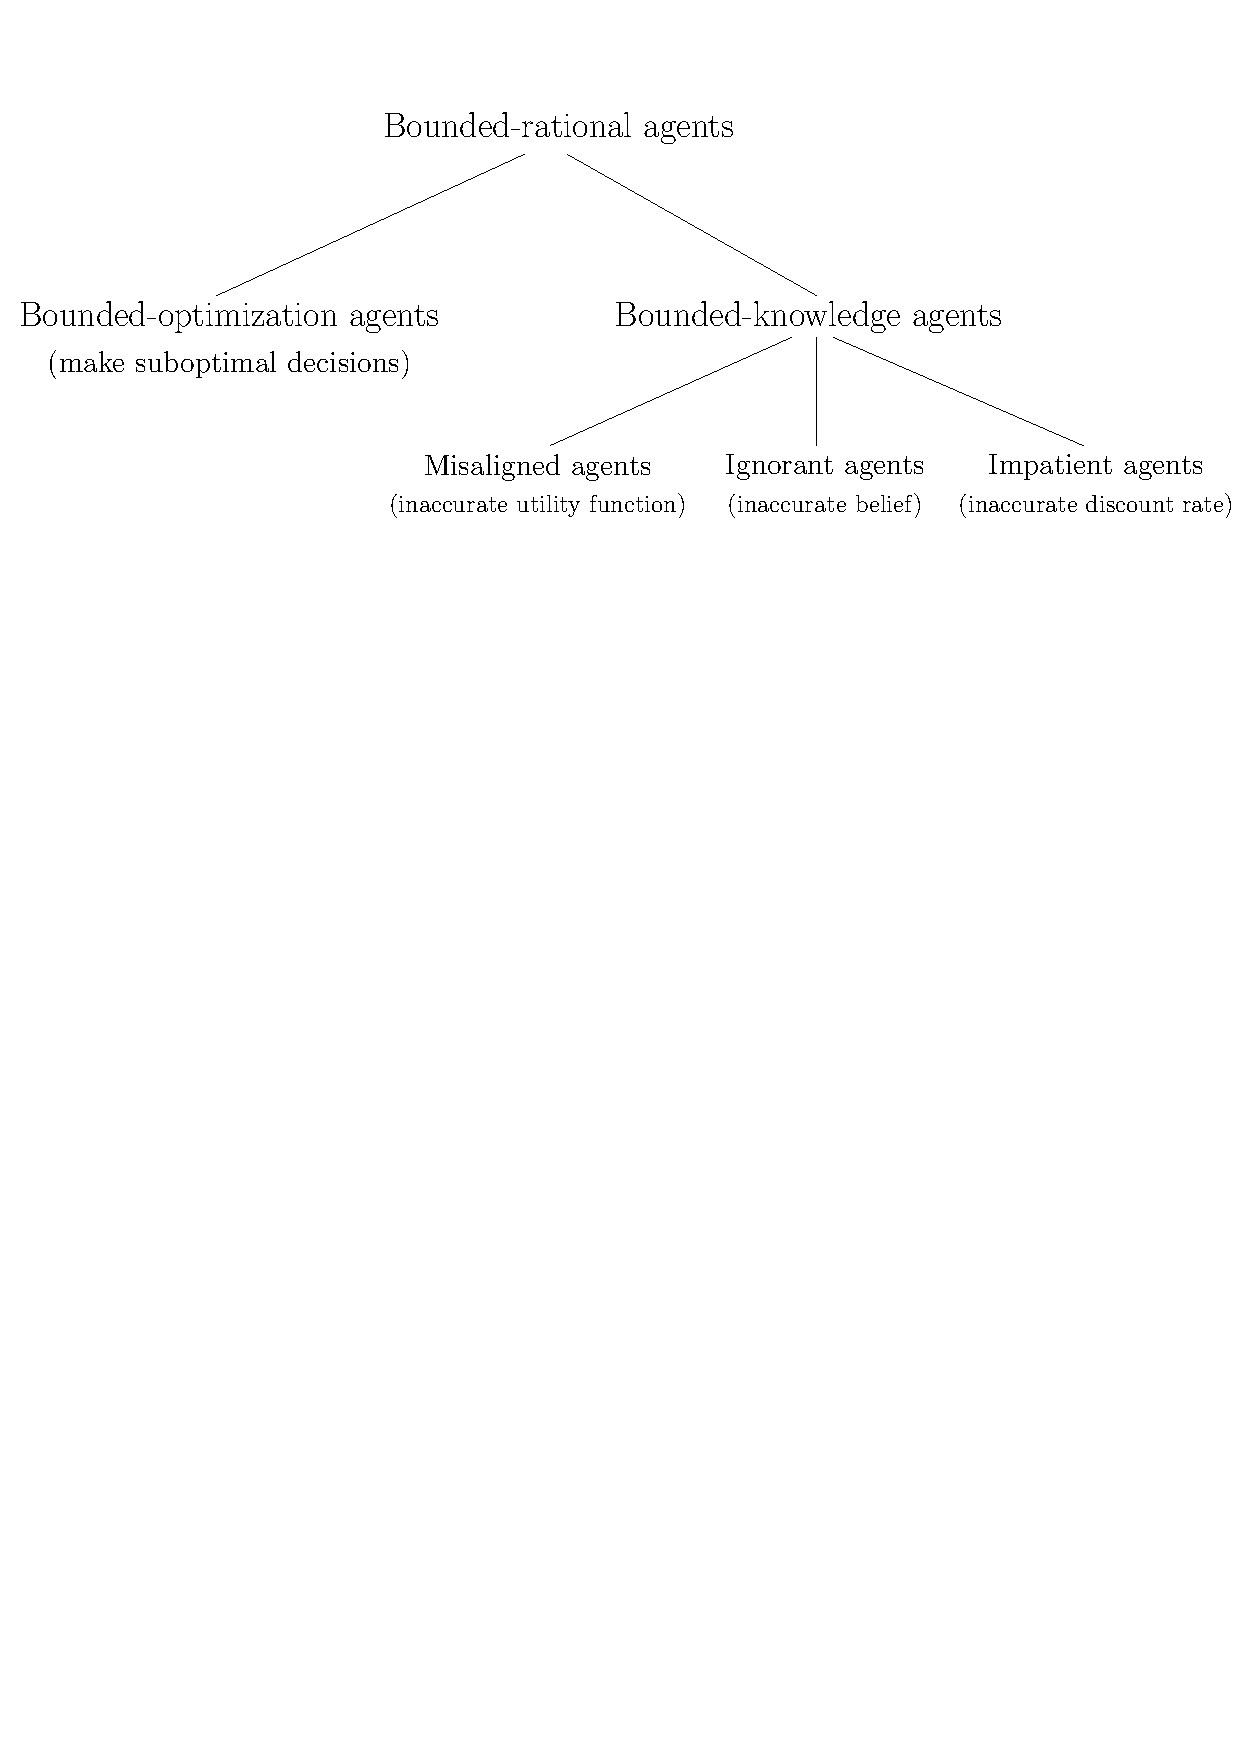
\includegraphics[width=13.7cm]{figures/agent_types_diagram}
\centering
\end{figure} %AAAI
%\end{figure*}

\subsection{Bounded-optimization agents} \label{sec:bounded_optimization}
We introduce the notion of \textit{$\epsilon$-optimizers}. Intuitively speaking, the expected future discounted utility gained by an $\epsilon$-optimizer is no more than $\epsilon$ lower than the optimal one in any situation they could get into (that is, for any history).
\begin{definition}
We say that agent $A$ is an $\epsilon$-optimizer for history $\mae_{<t}$ if it holds that 
\begin{equation} \label{eq:def_eps_opt}
Q(\mae_{<t}\pi(\mae_{<t})) \geq \sup_{\pi'} Q(\mae_{<t}\pi'(\mae_{<t})) - \epsilon
\end{equation}
\end{definition}

When the utility function, belief and discount factor is obvious from the context (or unimportant), we also speak of policy being $\epsilon$-optimizing (with respect to the utility function and belief), meaning that the corresponding agent is an $\epsilon$-optimizer.

%\begin{remark}
%We could also define a weaker version of $\epsilon$-optimization, where we would specify a set of histories, in which the inequality \ref{eq:def_eps_opt} would have to hold. We could then say that the \textit{agent is $\epsilon$-optimizing for that set of histories}. This would 
%\end{remark}

\subsection{Bounded-knowledge agents} 
We consider agents with inaccurate knowledge of the correct utility function (\Cref{def:inaccurate_utility}), inaccurate knowledge of the world (\Cref{def:inaccurate_belief_abs,def:inaccurate_belief_rel}), and inaccurate knowledge of the correct discount factor (how much future reward is worth compared to reward in the present).

\subsubsection{Misaligned agents} %AAAI
%\paragraph{Misaligned agents}
We define $\epsilon$-misaligned agents as agents whose utility function $u$ has absolute error $\epsilon$ with respect to the correct utility function $u^*$. 
\begin{definition} \label{def:inaccurate_utility}
We say that the instantaneous utility function $u$ has absolute error $\epsilon$ with respect to the correct utility function $u^*$ if
\[
\sup_{t\in \mathbb{N},\mae_{<t}} |u(\mae_{<t}) - u^*(\mae_{<t})| = \epsilon 
\]
\end{definition}

\subsubsection{Ignorant agents} %AAAI
%\paragraph{Ignorant agents}
We define $\epsilon$-ignorant agents as agents whose belief $\rho$ has error (absolute or relative depending on the context) $\epsilon$ with respect to the correct belief $\rho^*$. 

For belief, we define both relative and absolute error. This is in contrast with utility, for which this does not make sense in our setting. This is because when one speaks of relative utility, one usually compares it to some default action of ``doing nothing" which we do not have.

\begin{definition} \label{def:inaccurate_belief_abs}
We say that a belief $\rho$ has absolute error $\epsilon$ with respect to the correct belief $\rho^*$ if for any $t \in \mathbb{N}$, history $\mae_{<t}$ and action $a$,
\begin{align} 
\|\rho(\mae_{<t}a) - \rho^*(\mae_{<t}a)\|_{TV} \leq \epsilon\tag{$\star$}
\end{align}
where $\|\bullet\|_{TV}$ is the total variational distance. 
\end{definition}
Recall that (on discrete measure spaces where all subsets are measurable) for two distributions (formally two probability measures) $\mu$, $\nu$ on $\mathcal{E}$, the total variational distance is defined as
\[
\|\mu - \nu\|_{TV} = \sup_{E \subseteq \mathcal{E}} |\mu(E) - \nu(E)|
\]
\begin{definition} \label{def:inaccurate_belief_rel}
We say a belief $\rho$ has relative error $\epsilon$ with respect to the correct belief $\rho^*$ if for any $t \in \mathbb{N}$, any history $\mae_{<t}$, action $a$, and percept $e$,
\begin{equation}
\frac{1}{1+\epsilon} \leq \frac{\rho(e|\mae_{<t}a)}{\rho^*(e|\mae_{<t}a)} \leq 1+\epsilon
\end{equation}
\end{definition}

\paragraph{Impatient agents}
We define impatient agents as agents whose discount factor $\gamma$ is smaller than the correct discount factor $\gamma^*$. This means they have a stronger preference for immediate reward compared to the same reward in the future.
